\section{Galimi kodo skirstymo į paketus šablonai}
Diskusijose, kaip reikėtų skirstyti programinį kodą, paprastai akcentuojami du metodai - pagal \textit{techninį sluoksnį},
kur kiekvienam funkcionalumui arba kompiuterinės sistemos sluoksniui yra sukuriamas paketas,
grupuojant skirtingų dalykinių sričių esybes, arba pagal \textit{dalykinės srities esybes}, kur vienos esybės kodas, dalykinės srities
esybės funkcionalumas skirtingose programiniuose sluoksniuose yra patalpintas viename pakete~\cite{PackagingWays}
Tačiau šie du metodai yra gan platūs ir, dažniausiai jų nėra griežtai laikomasi - klasės būna išskaidytos remiantis papildomomis taisyklėmis,
siekiant išspresti sistemos planavimo metu kylančias problemas.
Norint išskirti šias papildomas taisykles, šablonus, buvo nagrinėjamos atviro kodo sistemos,
stebimi nukrypimai nuo bendresnio kodo skirstymo būdo ir identifikuojami klausimai arba problemos, kurias buvo bandoma išspresti.
\subsection{Sistemų analizės procesas}
todo: išsiplėsti apie sistemų analizės procesą


\subsection{Problemos}
Iš analizuotų sistemų buvo rastos šios problemos, būdingos sistemų dizainui, kartu su jas sprendžiančiais šablonais ir pavyzdžiais,
kokiose sistemose jie yra:

\subsubsection{Pagalbinių, daugkartinio naudojimo klasių skirstymas}
Pagalbinės ir daugkartinio naudojimo klasės dažniausiai negali būti patogiai grupuojamos skirstant pagal domeno esybes - pagalbines klases gali
naudoti kelios esybės, todėl neaišku, prie kurios jas reikėtų priskirti. Skirstant pagal techninį sluoksnį, bazines pagalbines klases gali naudoti keli
sluoksniai.
Didžiausia problema, susijusi su pagalbinėmis klasėmis, kurios turėtų išspręsti dažnai sistemoje sutinkamas problemas -
inžinieriai, dirbantys prie sistemos nežino apie jų egzistavimą, todėl jų nenaudoja,
tai veda prie didesnio kodo pasikartojimo arba kelių skirtingų to paties pagalbinio funkcionalumo įgyvendinimo.

\begin{figure}[H]
\snugshade
\dirtree{%
    .1 {/} .
    .2 {users} .
    .3 {UserRolesGrouping} .
    .3 {ArrayGroupingHelper} .
    .2 {\ldots} .
    .2 {payments} .
    .3 {PaymentScheduler} .
    .2 {\ldots} .
    .2 {transactions} .
    .3 {TransactionBatching} .
    .3 {utils} .
    .4 {ArrayGroupByUtil} .
}
\endsnugshade
\caption{Sistemos pavyzdys, kur labai panašią funkciją atliekančios klasės \textit{ArrayGroupByUtil} ir \textit{ArrayGroupingHelper}
egzistuoja todėl, kad inžinierius nerado jau įgyvendintos klasės, dėl aiškios struktūros daugartinio
panaudojimo klasėms trūkumo.}
\end{figure}
Vienas iš šablonų, sprendžiančių šią problemą, galėtų būti turėti vieną paketą, skirtą visoms pagalbinėmis klasėmis, kuris yra paminėtas sistemos
dokumentacijoje ir apie jo egzistavimą teoriškai žino visi komandos nariai.
Pakete reikėtų turėti atskiras klases kiekvienam bendriniam domenui, iš kurios pavadinimo programuotojas galėtų nuspresti,
kad jo ieškomas funkcionalumas, bus būtent toje klasėje.

\begin{figure}[H]
\snugshade
\dirtree{%
    .1 {/} .
    .2 {users} .
    .3 {UserRolesGrouping} .
    .2 {\ldots} .
    .2 {payments} .
    .3 {PaymentScheduler} .
    .2 {\ldots} .
    .2 {transactions} .
    .3 {TransactionBatching} .
    .2 {common} .
    .3 {Arrays} .
    .3 {Maps} .
    .3 {SqlQueries} .
    .3 {Users} .
}
\endsnugshade
\caption{Sistemos pavyzdys, kur visas bendrinio panaudojimo kodas guli \textit{common} pakete, pirmame sistemos paketų lygyje, todėl
pagalbinės klasės yra lengvai randamos.}
\end{figure}

Jei pagalbinių klasių dydis labai išauga, jas galima sumažinti ir vietoj vienos atskiros klasės vienai bendrinei sričiai, sukurti vieną paketą,
ir jame turėti kelias pagalbines klases, susijusias su tuo domenu.
Tokiu atveju reikia užtikrinti, kad iš klasių pavadinimo aišku, kokį srities subdomeną padengia klasė.
\begin{figure}[H]
\snugshade
\dirtree{%
    .1 {/common} .
    .2 {arrays} .
    .3 {ArrayFilters} .
    .3 {ArrayComparators} .
    .2 {\ldots} .
    .2 {maps} .
    .3 {MapTransformations} .
    .3 {MapJoining} .
    .2 {json} .
    .3 {JsonParser} .
    .2 {\ldots} .
    .2 {database} .
    .3 {DatabaseConnection} .
    .3 {DatabaseQueries} .
}
\endsnugshade
\caption{Sistemos pavyzdys, kur bendrinio panaudojimo kodas guli \textit{common} pakete, po domeno subpaketais, taip sumažinant klasių dydį }
\end{figure}

Tokį pagalbinių klasių skirstymo metodą naudoja keletas repozitorijų - pavyzdžiui, užrašinės aplikacijos \textit{Omni-Notes}\footnote{\url{https://github.com/federicoiosue/Omni-Notes/tree/develop/omniNotes/src/main/java/it/feio/android/omninotes/utils}} bei
\textit{Fire Sticker}\footnote{\url{https://github.com/hackjutsu/Fire_Sticker/tree/master/app/src/main/java/com/gogocosmo/cosmoqiu/fire_sticker/Utils}}

Naudojant tokį šabloną, programuotojas, susiduriantis su bendrine problema, kuri, labai tikėtina, jau yra išspręsta sistemoje turėtų
aiškų procesą, kaip elgtis šioje situacijoje:
\begin{enumerate}
    \item Atsidaryti vieną paketą, skirtą bendrinio panaudojimo kodui
    \item Pakete surasti klasę, kurios pavadinimas būtų susijęs su jo problema
    \item Klasės funkcijų saraše surasti jam tinkamą funkciją.
    \item Jei reikalingas funkcionalumas nerastas, įgyvendinti jį pasirinktoje klasėje, padengti jį testais,
    bei aprašyti dokumentaciją, kaip funkcija turėtų būti naudojama.
    \item Iškviesti rastą arba sukurtą funkciją iš bendrinio panaudojimo kodo paketo savo funkcionalume
\end{enumerate}

\subsubsection{Ka daryti esant dideliam priklausomybių nuo paketo skaičiui?}
Didelis priklausomybių nuo specifinio paketo skaičius (arba aferentinės jungtys), reiškia, kad pokyčiai tame pakete turės įtaką kelioms klasėms.
Jei tokia tendencija yra būdinga visai sistemai, sistema tampa mažiau lanksti pokyčiams, kadangi net ir paprastas pakeitimas
daro įtaką reišmingai sistemos daliai, pokyčiai yra labiau linkę keisti bendrą sistemos architektūrą.
Taip pat naujos sistemos versijos išleidimo \angl{release} procesas tampa sudetingesnis, kadangi yra paveikiama daugiau klasių.

Robert C. Martin bendro sąryšio principas, kuris teigia, kad visos tarpusavyje susijusios klasės turėtų būti vienam pakete,
akcentuoja siekiamybę turėti gan mažus paketus, turinčius aiškiai apibrėžtą funkcionalumą, priežastį egzistuoti, taip užtikrinant
glaudų tarpusavyje susijusių klasių saryšį.
Šis principas galėtų būti kodo skirstymo šablonas, užtikrinantis racionalų aferentinių jungčių skaičių paketuose.

Vadovaujantis šiuo šablonu kiekvieną paketą reikėtų realizuoti kaip komponentą, teikiantį vieną funkcionalumą.
Funkcionalumas kitiems paketams yra pasiekiamas per vieną minimalią sąsają \angl{interface},
kuri atskleidžia tik konceptus (metodus arba duomenų tipus), kurie yra glaudžiai susiję su komponento teikiama paslauga, bei
klase, gražinančią minėtos sąsajos įgyvendinimą.
Tai gali būti paprasta klasė, su statine funkcija, kurios rezultatas yra ši sąsaja, arba, esant keliomis sąsajos implementacijomis,
\textit{Static factory} dizaino šablonas, kuris nusprendžia kuri įgyvendinimą reiketų grąžinti pagal paduotus argumentus.

Visos kitos klasės naudoja \textit{package} pasiekiamumo modifikatorių, taip kompiliatoriaus pagalba užtikrinant,
kad jos nebus pasiektos iš išorės.

Paketas turintis vieną funkciją yra naudojamas tik tų paketų, kuriems reikia būtent tos funkcijos,
taip užtikrinant tik mažos sistemos dalies priklausomybę nuo vieno paketo.

Toks konceptas yra sutinkamas \textit{Typescript} programavimo kalboje, kur kiekvienas modulis (šios kalbos paketo atitikmuo) turi
\textit{index.ts} faila, veikiantį kaip sąsaja, apibrėžiančia, kokios modulio klasės bei funkcijos gali būti pasiekiamos už paketo ribų.
Tai užtikrina glaustą kontraktą ir aiškų modulio funkcionalumą, kurį gali pasiekti kiti moduliai, bei paslepia modulio įgyvendinimo detales.
Toki šabloną naudoja turinio valdymo sistema \textit{Keystone}\footnote{\url{https://github.com/keystonejs/keystone/tree/main/packages/core/src/fields/types}},
kur kiekvieną esybė turi savo modulį, atliekantį vieną funkcija, kurio kontraktas aprašytas \textit{index.ts} faile.

\begin{figure}[H]
    \snugshade
    \dirtree{%
        .1 {/types} .
        .2 {image} .
        .3 {views} .
        .3 {utils} .
        .3 {index} .
        .2 {text} .
        .3 {views} .
        .3 {index} .
        .2 {...} .
        .2 {checkbox} .
        .3 {views} .
        .3 {index} .
    }
    \endsnugshade
    \caption{\textit{Keystone} sistemos dalis, kurioje matomi smulkūs moduliai su \textit{index.ts} failuose aprašytais kontraktais}
\end{figure}

Taip pat mažas paketo funkcionalumas reiškia, kad minėtas paketas skirtas funkcionalumui įgyvendinti naudos minimalų kitų sistemos esybių skaičių,
taip sumažinant ir eferentinių jungčių skaičių.

Žemiau esančiuose paveikslėliuose galima matyti, kaip išskaidant paketus, turinčius kelis funckionalumus, yra sumažinamas paketų
priklausomybių skaičius.
\begin{figure}[H]
    \centering
    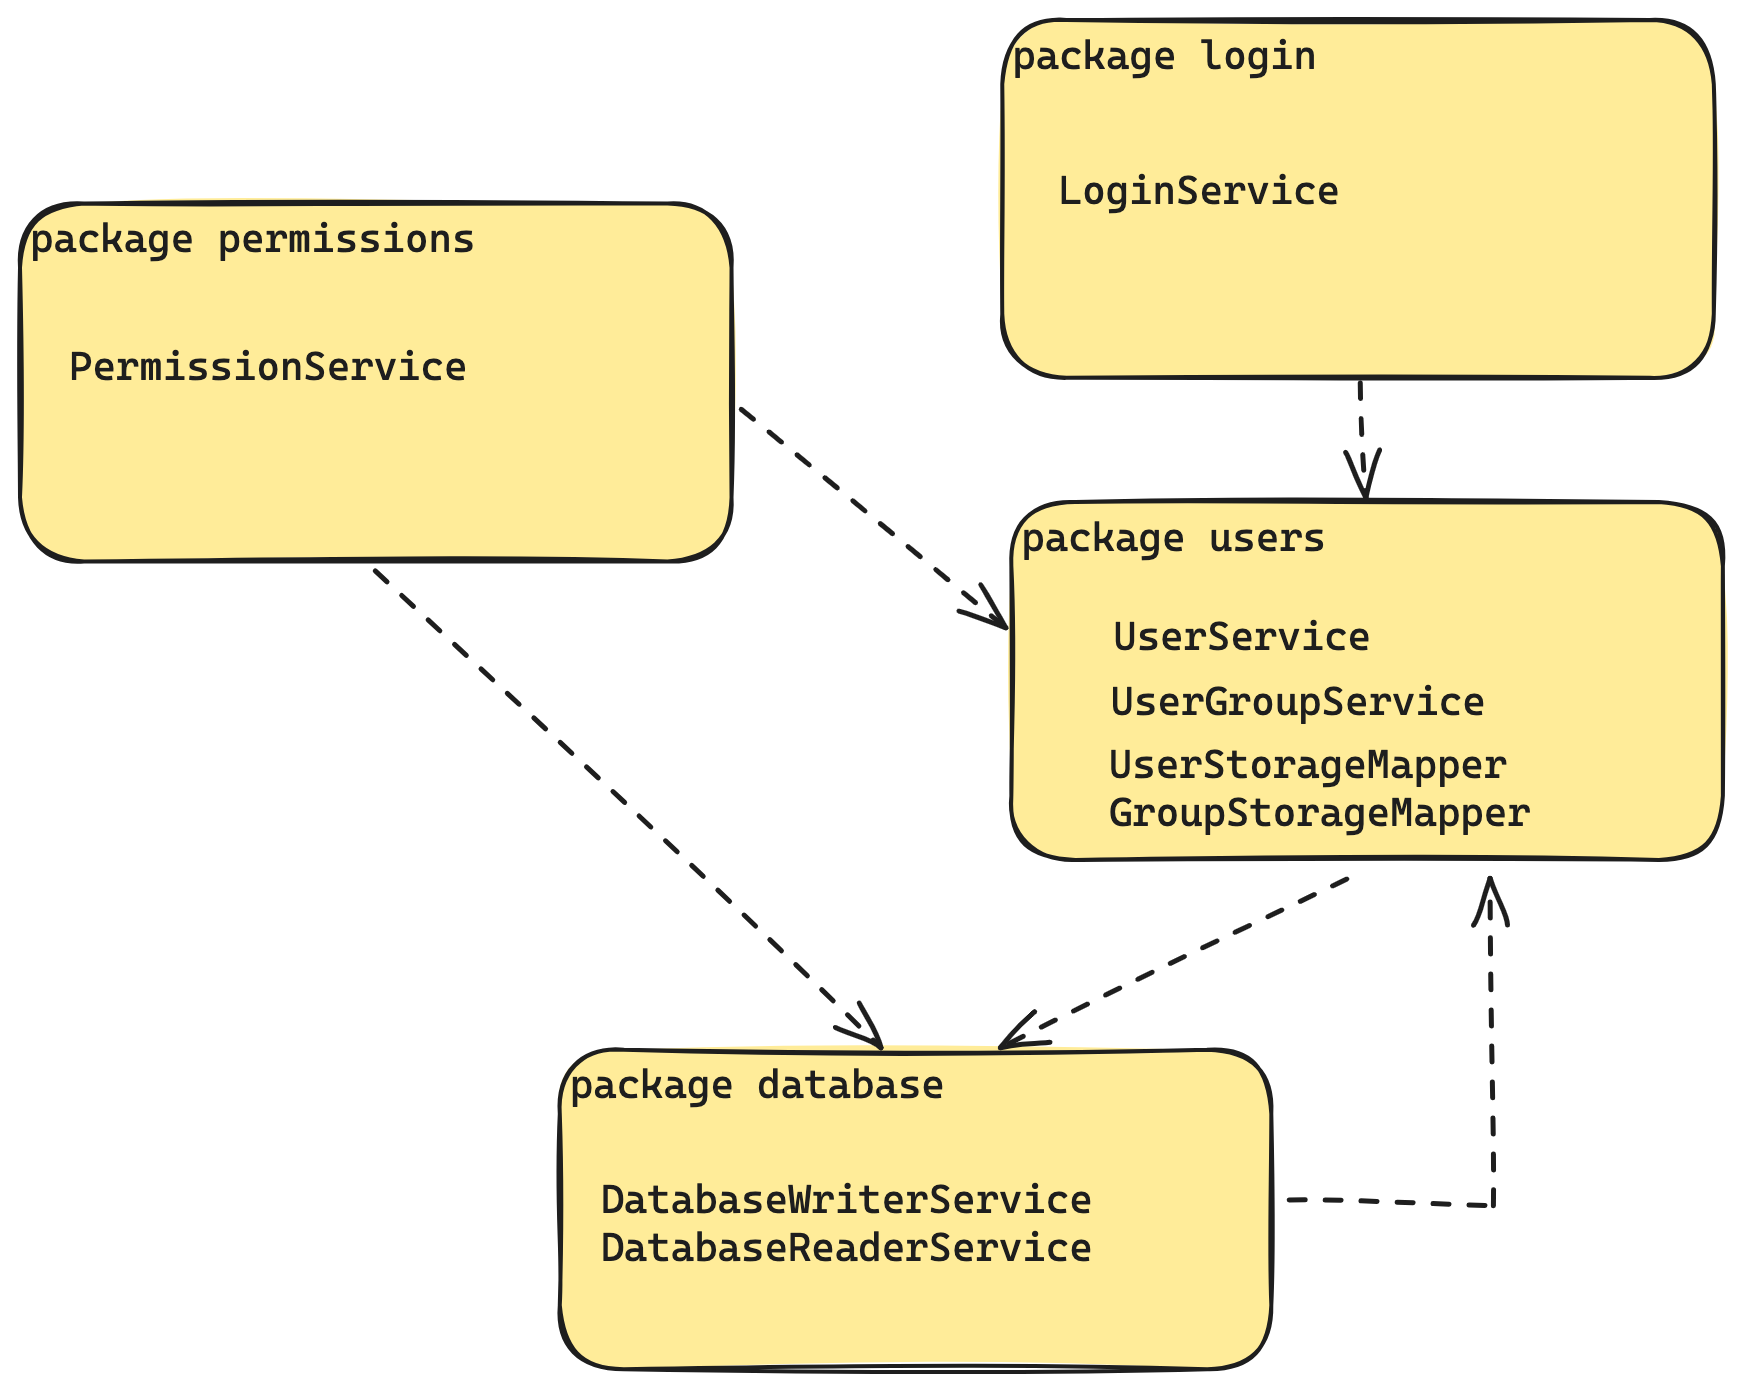
\includegraphics[scale=0.15]{img/excesive_deps}
    \caption{Sistemos pavyzdys su kelias funkcijas atliekančiais paketais}
    \label{img:excesive_deps}
\end{figure}


\begin{figure}[H]
    \centering
    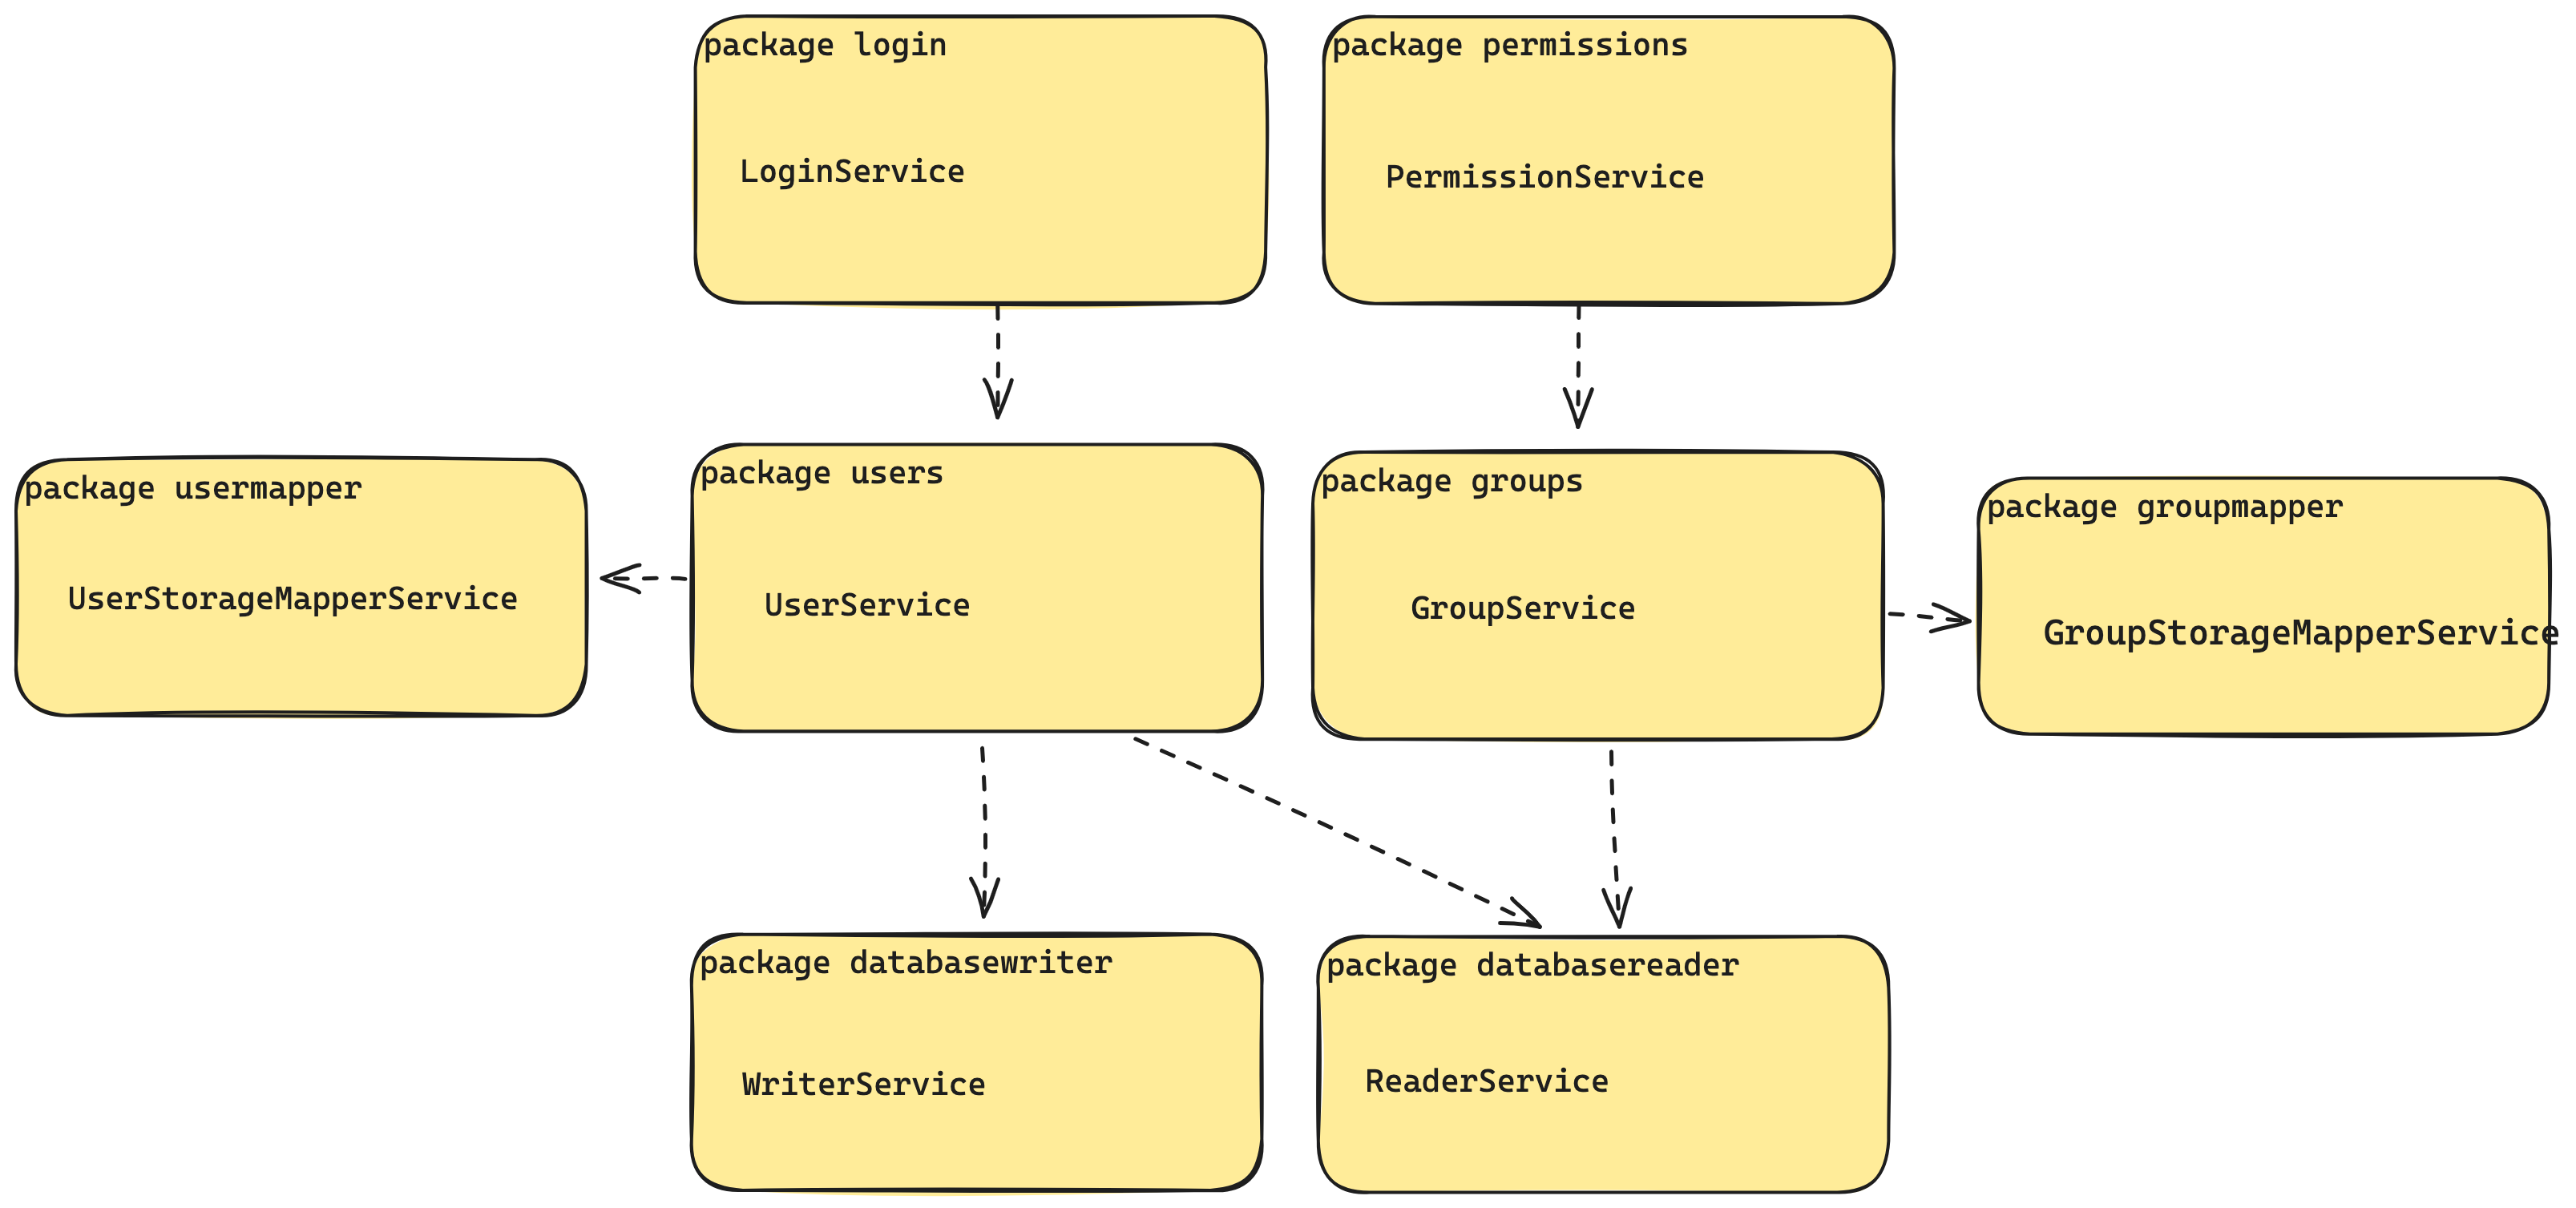
\includegraphics[scale=0.13]{img/good_deps}
    \caption{Sistemos pavyzdys su aiškią, vieną funkciją turinčiais paketais}
    \label{img:good_deps}
\end{figure}

Toks skirstymo būdas taip pat sprendžia ciklinių priklausomybių problemą - pavyzdžiui, įrankio, skirto spręsti ciklinių priklausomybių problemą,
kūrimo aprašas~\cite{CircularDependencies} teigia, kad ciklinių priklausomybių problemą galima spręsti laikantis trijų principų -
bendro panaudojimo, bendro keitimosi bei paleidimo ir pernaudojimo ekvivalentumo.
Šie principai yra išvesti iš bendro saryšio principo ir akcentuoja, kad kartu besikeičiančios klasės turėtų būti viename pakete.
Norint užtikrinti šiuos reikalavimus, reikėtų turėti mažą,
tiksliai apibrėžto funkcionalumo paketą, kurio visi komponentai - tarpusavyje susiję.
Tokiu atveju ciklinių priklausomybių tikimybė sumažėja.

\subsubsection{Ka daryti su daug skirtingų sąsajų implementacijų?}
Sistemai plečiantis, galima susidurti su problema, kad išauga sąsajos implementacijų skaičius. Ši problema gali iškilti
tiek bandant skirstyti kodą pagal domeno esybes, tiek pagal techninį sluoksnį. Skirstant pagal domeną, gali būti neaišku, kur turėtų
būti sukuriamas naujas esybės paketa. Skirstant kodą pagal techninį sluoksnį, gali susidaryti klasių perteklius, pavyzdžiui,
model pakete. Tokiu atveju navigacija pakete pasidaro sudėtinga, neaišku, kas implementuoja.
Šią problemą būtų galima spręsti sukuriant sąsajos implementacijas tame pačiame pakete kaip ir pati sąsają.
Toks skirstymo į paketus šablonas yra sutinkamas \textit{Java} standartinėje bibliotekoje\footnote{\url{https://github.com/AdoptOpenJDK/openjdk-jdk11/tree/master/src/java.base/share/classes/java/util}},
kur visos standartinės sąsajos bei jų implementacijos yra tame pačiame pakete.
Dėl tokios paketų struktūros, inžinieriai, naudojantys standartinę \textit{Java} biblioteką, gali lengvai rasti jiems reikiamus sąsajos įgyvendinimus:
\begin{figure}[H]
    \snugshade
    \dirtree{%
        .1 {/util} .
        .2 {Map} .
        .2 {HashMap} .
        .2 {LinkedHashMap} .
        .2 {WeakHashMap} .
        .2 {TreeMap} .
        .2 {...} .
        .2 {List} .
        .2 {LinkedList} .
        .2 {ArrayList} .
    }
    \endsnugshade
    \caption{\textit{Java} standartinės bibliotekos pavyzdys, kuriame sąsajų įgyvendinimai guli tame pačiame pakete, kaip ir sąsajos}
\end{figure}
Taip pat, jei viena sąsaja turi labai daug implementacijų, norint padaryti paketo turinį aiškesnį, galima sukurti po subpaketą
specifinės sąsajos implementacijoms.
\begin{figure}[H]
    \snugshade
    \dirtree{%
        .1 {/util} .
        .2 {Map} .
        .2 {map} .
        .3 {HashMap} .
        .3 {LinkedHashMap} .
        .3 {WeakHashMap} .
        .3 {TreeMap} .
        .2 {...} .
        .2 {List} .
        .2 {list} .
        .3 {LinkedList} .
        .3 {ArrayList} .
    }
    \endsnugshade
    \caption{\textit{Java} standartinės bibliotekos pavyzdys, jei kiekvienai sąsajai būtų sukurtas subpaketas, jos įgyvendinamams laikyti}
\end{figure}

\subsubsection{Kaip valdyti esybių pokyčius ir versijavimą}
Sistemai egzistuojant ilgesnį laiką, jos pokyčiai pasidaro neišvengiami.
Smulkūs pokyčiai nebūtinai paveikia bendrą sistemos struktūrą, tačiau
didesniems pokyčiams kartais reikia sukurti naujas klasių ar funkcionalumų versijas. Jei reikia palaikyti atgalinį
suderinamumą (angl. backward compatibility), sistemoje gali atsirasti kelios tų pačių esybių versijos.
Tokiu atveju kelios tų pačių esybių versijos sistemoje gali pridėti painumo.
Ši problema dažnai sprendžiama sukuriant atskirus paketus skirtingoms
versijoms (v1, v2, v3, \ldots) bei iškeliant bendrą, abiejų esybių naudojama kodą į subpaketus taip, kad jas galėtų pasiekti abi versijos.
Taip galima išvengti kodo duplikacijos bei perteklinio klasių skaičiaus paketuose, bei užtikrinant aiškia skirtingų versijų
atskirti.
\begin{figure}[H]
    \snugshade
    \dirtree{%
        .1 {/regex} .
        .2 {common} .
        .2 {pending} .
        .2 {v3} .
        .2 {v4} .
        .2 {...} .
    }
    \endsnugshade
    \caption{\textit{Mongo} duombazės Sistemos pavyzdys, kurioje skirtingos versijos patalpintos atskiruose paketuose}
\end{figure}
Toks skirstymo būdas matomas keliose repozitorijose - \textit{Mongo}\footnote{\url{https://github.com/mongodb/mongo/tree/master/src/third_party/boost/boost/regex}} duomenų bazėje,
API skirtame kelionių valdymui \textit{travels-java-api}\footnote{\url{https://github.com/mariazevedo88/travels-java-api/tree/master/src/main/java/io/github/mariazevedo88/travelsjavaapi/controller}}
 bei duomenų saugojimo įrankyje \textit{nocodb}\footnote{\url{https://github.com/nocodb/nocodb/tree/c7cc1f92fd77f8b5daefceb7148aab4a69cb9b4e/packages/nocodb/src/meta/migrations}}.
Šiose repozitorijose v1, v2 pavadinti paketai saugo skirtingas esybių versijas.